Welcome to the fifth instalment of Adventures in Recreational Mathematics! This article is about Cantor's work on the puzzling subject of infinity. He believed it came from God, but Cantor and his work were attacked by such people as Wittgenstein, calling it ``utter nonsense",  Poincare, who said it was ``a disease infecting mathematics" and worst of all Kroenecker, who described him as ``a corrupter of youth, a scientific charlatan". Despite these fierce attacks from Premier League detractors, today his work is generally accepted - read on to see what you make of his revolutionary and counter intuitive ideas.

We begin with the concept of an ordering. A set is a collection of objects; those objects can be "ordered" according to some relation - for example we can sort them by size, by age, alphabetically etc. Formally this is stated as a binary relation \(\curlyeqprec\) relating two objects in a set (i.e. \(x\curlyeqprec y\)) so that for all elements \(a, b, c\) in the set it satisfies these three axioms:

1. \( a \curlyeqprec a \) (reflexivity)

2. If \( a \curlyeqprec b \) and \(b \curlyeqprec a \), then \(a = b\) (antisymmetry)

3. If \( a \curlyeqprec b \) and \(b \curlyeqprec c \), then \(a \curlyeqprec c \) (transitivity)

\(\curlyeqprec\) places the objects of a set into a hierarchy. \(\curlyeqprec\) is called a \textit{partial order} and the set it governs is naturally called a \textit{partially ordered set (poset)} - an example would be the relation \(\leq\) on the set of numbers.

To demonstrate how partial orders don't have to exhibit a linear hierarchy, we can visualise posets using \textit{Hasse diagrams}, for which the rules of construction are to draw a node for every element of the poset and then draw a line \textit{upwards} (possibly diagonally upwards) from an element \(x\) to an element \(y\) if \(x \curlyeqprec y \) and there is no element \(z\) such that \(x \curlyeqprec z \curlyeqprec y\) (as in these cases, \(x \curlyeqprec z\) is represented on the diagram, as is \(z \curlyeqprec y\), so we can work out that \(x \curlyeqprec y\)). Below, in Fig. 1, we can see two such diagrams: the leftmost displays the set of factors of 120, where \(x\curlyeqprec y\) if \(x\) is a factor of \(y\), and the rightmost shows the set of all subsets of \(\{2, 3, 4, 5, 8\}\) such that if \(x\) is a member of one such subset then all members of \(\{2,3,4,5,8\}\) which are factors of \(x\) are also in the subset, ordered by set inclusion.

\begin{figure}[h]
\centering
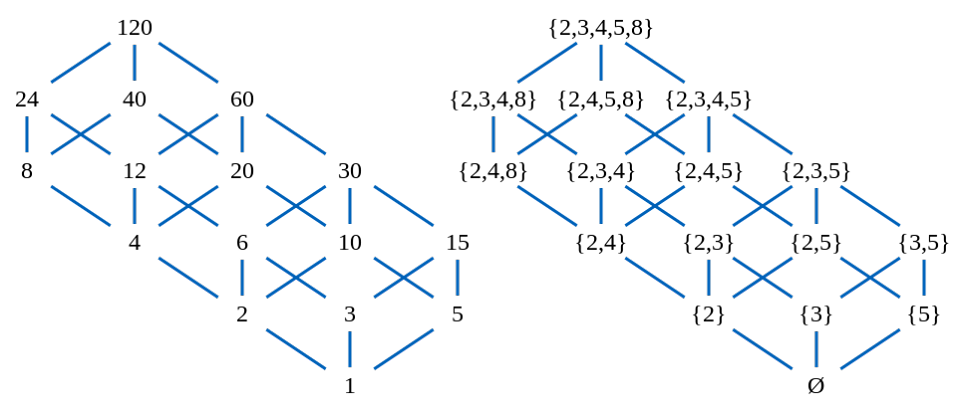
\includegraphics{graph}
\caption{An example of order isomorphism}
\end{figure}

Do you notice anything interesting? Although the subject matters of the posets are quite different, their Hasse diagrams and thus their orderings appear to have, in some sense, the same structure. To be more precise, let's consider two posets \((S, \curlyeqprec_S)\) and \((T, \curlyeqprec_T)\). A bijective function (a one-to-one mapping between the elements of two sets) \(f\) from \(S\) to \(T\) is called an \textit{order isomorphism} if \( x, y \in S, x \curlyeqprec_S y\) implies \( f(x) \curlyeqprec_T f(y) \) and vice versa; the existence of such a function means that \(S\) and \(T\) are \textit{order isomorphic}. This is an important concept, as we will soon see.

\textit{Well-orders} paired with \textit{well-ordered sets (wosets)} make up a subset of partial orders \& posets which further follow these axioms: for any two elements \(a, b\) of a woset \((W, \curlyeqprec_W)\), at least one of \( a \curlyeqprec_W b\) or \(b\curlyeqprec_Wa\) is true and for any \(G \subseteq W \), there is an element \(c \in G \) which is ``below'' in the ordering any other element of \(G\) (i.e. there is always a least element). These properties of relations are called totality and well-foundedness respectively. Can you guess what the Hasse diagrams of wosets look like?

To visualise this more easily, a classic example of a well-ordered set is the natural numbers with \( \leq \) as the ordering - this observation is called the \textit{Well-Ordering Principle} and is quite interesting, since it turns out that this statement is equivalent to the assertion of the validity of \textit{induction}. In fact, the famous set-theoretic \textbf{Axiom of Choice} asserts that \textit{any set can be well-ordered}, which despite seeming obvious in principle is in practise impossible to prove using just the axioms of ZF set theory (one of the modern-day formulations of set theory, designed to avoid logical paradoxes).

Cantor discovered all of this and observed something: since the structure of well-orderings is essentially linear, it might be possible to define an infinite set (more specifically, a \textit{proper class}) \(S\) of sets increasing in size such that every well-ordered set is order isomorphic to exactly one member of \(S\). Cantor (and subsequently \textit{John von Neumann}, whose definition we will be using) did just that and these sets are called \textbf{the ordinals}:

1. \(\emptyset\) (the empty set) is an ordinal.

2. Ordinals are well-ordered by the relation \( \subseteq \).

3. Every ordinal is the set of all ordinals "below" or smaller than it.

Due to them being order isomorphic, most people notate finite ordinals as the natural numbers, referring to them as the ``ordinal numbers", along with common use of \(\leq\) and \(<\) in notation, so \[ \emptyset = 0, \{0\} = 1, \{0, 1\} = 2, ... \]

The ordinal that a given well-ordered set is order isomorphic to is called the \textit{order type} of that set. There are many nice properties that immediately spring from this definition: a given ordinal \textit{is} the set of all those below it, there are an infinite number of ordinals and more ... Interestingly, it shows that there cannot be what Cantor called \(\Omega\), the set of all ordinals, since such a set would have an order-type \(\delta\) larger than \(\Omega\) since \(\Omega\) \textit{is an ordinal}. However, \(\delta\in\Omega\) and thus \(\delta\) would have to be bigger than itself - this contradiction means that such a set cannot exist. Cantor, however, was a deeply religious man who connected \(\Omega\) philosophically with God as ``the absolute infinite", a quantity bigger than anything conceivable or inconceivable, and so simply concluded that ``\(\Omega\)'s nature is contradictory'' and is perhaps \textit{beyond mathematics}. Today we say that there is a \textit{class} of ordinals but not a set: every property that a mathematical object (like a number) can have defines a class of objects with that property, every set is a class but the converse is not true; this removes many paradoxes such as the Russell Paradox posed to set theorists at the end of the 19th century.

There are 3 types of ordinals: 0, successor ordinals and limit ordinals. An ordinal is a \textit{successor ordinal} if, for some \(a\), it can be represented as the set \(\{ x | x\leq a \}\) or, equally, \( a \cup \{a\}\) - the intuitive way of thinking about this is that successor ordinals are just one plus some other ordinal (so far, this isn't very different from the natural numbers). An ordinal \(b\) is a \textit{limit ordinal} if for every set element \(s_0 < b\), there exists an \(s_1\) so that \(s_0<s_1<b\) - it should soon become apparent that limit ordinals are what most people would call ``infinities"!

Another way of seeing limit ordinals is as limits of a sequence: if we have a strictly increasing sequence of ordinals \(\langle a_i | i < G \rangle\) (this is the notation for sequences of ordinals) where \(G\) is a limit ordinal, then we say that the \textit{limit} of that sequence is the smallest ordinal greater than all those in the sequence. Limit ordinals can thus be seen as the limit of the sequence formed by all those ordinals below them. Moreover, such a limit \textbf{always exists}! The existence of limit ordinals has many consequences, a few of which we will explore now.

Consider the sequence \(1, 2, 4, 8, 16, 32, ..., 2^n, ...\). Remarkably, this does have a limit, \textbf{\(\omega\)}, the first limit ordinal! This number is above all of the integers and, by the definition of ordinals, is the set of natural numbers. Cantor called \(\omega\) a \textit{transfinite number}, since although it is above all the finite numbers, it isn't above \(\Omega\). There must be a successor cardinal to \(\omega\), namely \(\omega + 1\), which is a distinct ordering from that of the natural numbers since it has a \textit{greatest element}! This too has a successor \( \omega + 2\) and so on: \( \omega + 3, \omega+4, ..., \omega +5\); remember that this is a strictly increasing sequence and so must have a limit, which is \( \omega\times{}2\).

Further, ZF set theory's \textbf{Axiom of Comprehension} states that if one has a \textit{well-defined property} \( \phi (x) \) (this notation simply denotes \(x\) having that property) then there exists a class of objects with that property. This means we can define \( \Lambda \) to be the class of all limit ordinals and then, by well-ordering it, we can talk of the sequence \(\langle a_i | i \in \Lambda, i < j \Rightarrow a_i < a_j \rangle\). This must have a limit and we will call it \( \lambda\): the limit of all limit ordinals (which is itself a limit ordinal).

Ordinals clearly have complex properties but to truly be able to investigate them in depth, we need to consider how one can define a \textit{class function} over the ordinals. One must begin by understanding transfinite induction: to prove a property \( \phi(x)\) holds for all ordinals we need to prove \(\phi(0)\) holds (the so-called \textit{base case}), we then must show that \(\phi(a) \Rightarrow \phi (a+1) \) (the inductive step) and finally we must show that for any limit ordinal \(\gamma\), \([\phi(x)\) for all \(x<\gamma] \Rightarrow \phi(\gamma)\). Usually a proof by induction involves just the first two steps; the third step is needed here because limit ordinals aren't the direct successor to any particular number and so the second inductive step doesn't reach them. This turns out to be incredibly useful since it allows us to prove a result known as \textit{transfinite recursion} - any class function \(f(x)\) defined in reference to \(f(a)\) for all \(a<x\) is unique and well-defined!

Now we can completely (inductively) define arithmetic on ordinals. Let's begin with addition:

1. \(a + 0 = a\)

2. \((a+b)+1 = a+(b+1)\) (the \(+1\) denotes the successor ordinal)

3. For a limit ordinal \(\gamma\), \(a+\gamma\) is the limit of the sequence \(\langle a+i | i < \gamma \rangle\)

You can understand \(a+b\) by considering \(a\) and \(b\) as two disjoint ordered sets, \((S_a,\curlyeqprec_a)\) and \((S_b,\curlyeqprec_b)\), taking their union \(S_{a+b}\) and then imposing a new order \(\curlyeqprec_{a+b}\) so that: the ordering of \(S_a\)'s and \(S_b\)'s elements are kept the same and all elements in \(S_b\) are above \(S_a\) in the ordering, like this with the example of \(2+3\): \[ 0_a\curlyeqprec_{a+b}1_a\curlyeqprec_{a+b}0_b\curlyeqprec_{a+b}1_b\curlyeqprec_{a+b}2_b \] This chain of 5 elements is order isomorphic to the ordinal 5, since you can just relabel the elements with normal ordinal notation to get \[0<1<2<3<4\] This simple result allows us to see that \(1+\omega = \omega\) since these two never ending chains are order isomorphic: \[ 0_a\curlyeqprec_{a+b}0_b\curlyeqprec_{a+b}1_b\curlyeqprec_{a+b}2_b\curlyeqprec_{a+b}... \cong 0<1<2<3<... \] (where \(\cong\) denotes order ismorphism) However, \(\omega + 1\) is different as it has a final term or \textit{greatest element}: \( 0_a < 1_a < 2_a < ... < 0_b\). This non-commutative addition showing that \(1+\omega \neq \omega+1\) originally drew heavy criticism to Cantor. Next, we have the definition of multiplication, which is exactly what someone used to the hierarchy of \textit{hyperoperations} would expect:

1. \(a\times{}0 = 0\)

2. \(a\times{}(b+1) = (a\times{}b)+a \)

3. For a limit ordinal \(\gamma\), \(a\times{}\gamma\) is the limit of the sequence \(\langle a\times{}i | i < \gamma \rangle\)

\(a\times{}b\) can be understood by once again considering \(a\) and \(b\) as the two disjoint ordered sets \((S_a,\curlyeqprec_a)\) and \((S_b,\curlyeqprec_b)\), taking their \textit{cartesian product}, which is the set of all pairings of elements between \(a\) and \(b\), and then imposing an order \(\curlyeqprec_{a\times{}b}\) where an element \( (a_0, b_0) \) is below another element \( (a_1, b_1) \) if \( b_0 < b_1\) or if \(b_0 = b_1, a_0 < a_1\). For example, we can display \(2\times{}3\) in our previous intuitive ``order representation" as



\vspace{-2.5em}

\[ (0, 0) \curlyeqprec_{a\times{}b} (1, 0) \curlyeqprec_{a\times{}b} (0, 1) \curlyeqprec_{a\times{}b} (1, 1) \curlyeqprec_{a\times{}b} (0, 2) \curlyeqprec_{a\times{}b} (1, 2) \cong 0 < 1 < 2 < 3 < 4 < 5\]



Can you see what \(3\times{}2\) is and why it is order isomorphic to \(2\times{}3\)?

Just like ordinal addition, ordinal multiplication is not necessarily commutative (\(a\times{}b\) doesn't always equal \(b\times{}a\)) when we start dealing with transfinite numbers. For example, we can see from the inductive definition that \(2\times{}\omega = \langle 2\times{}i | i < \omega \rangle = \omega\) but \(\omega\times{}2 = \omega + \omega\), so \(2\times{}\omega \neq \omega\times{}2\). This can be represented as



\vspace{-2.5em}

\[ (0, 0) \curlyeqprec_{a\times{}b} (1, 0) \curlyeqprec_{a\times{}b} (0, 1) \curlyeqprec_{a\times{}b} ... \ncong (0, 0) \curlyeqprec_{a\times{}b} (1, 0) \curlyeqprec_{a\times{}b} (2, 0) \curlyeqprec_{a\times{}b} ... \curlyeqprec_{a\times{}b} (0,1) \curlyeqprec_{a\times{}b} (1,1) \curlyeqprec_{a\times{}b} ... \]



\(\omega\times{}2\) contains two unbounded sequences in front of each other, which is distinct from \(\omega\)'s single unbounded sequence.

It's not necessary to give the inductive definition of ordinal exponentiation here; it should be clear by now what it would be. From the order representation perspective, we would be simply dealing with longer \textit{tuples} (the ordered bracket groupings) in our sequences where the length of the tuples is dictated by the exponent and the maximum number that can be counted to in each entry is dictated by the base. So \(2^3\) can be seen as \( (0, 0, 0) \curlyeqprec_{a^b} (0, 0, 1) \curlyeqprec_{a^b} (0, 1, 0) \curlyeqprec_{a^b} (0, 1, 1) \curlyeqprec_{a^b} \) etc.

We now understand the concept of order types fairly well but is there another inherent distinguishing property of wosets that might be important? Size! You may have noticed that I often referred to a situation like \(a \curlyeqprec b\) as \(b\) being "above" \(a\) in an ordering, rather than "greater than" or "more than" - this is to distinguish between ordinality and size, or what Cantor called \textit{cardinality}. The distinction is not obvious on a finite scale, since the finite ordinal \(n\) has \(n\) elements, which is written \(|n| = n\), but Cantor's great observation was that infinite sets of the \textit{same cardinality} can have \textit{differing orderings}. So surely, if we are talking truly about \textbf{size}, then we don't need to worry about all the "bigger infinities" rhetoric - a set is either finite or infinite, right?

Wonderfully, amazingly, it is not so. To prove this, we first observe that one way of proving that two sets \(A\) and \(B\) have the same cardinality is to exhibit a one-to-one mapping between their elements, known, as we have seen above, as a bijective function, and that a way of proving that \(|A| \leq |B| \) is to exhibit an injective function from \(A\) to \(B\) (a function \(f\) is injective if for two inputs \(x, y\) where \(x \neq y\), \(f(x) \neq f(y)\)). Then, any set for which there exists an injective function from it to the set of natural numbers, \(\omega\), we shall call \textit{countable} and we can call \(\omega\) the first \textit{transfinite countable}, since other transfinite ordinals like \(\omega\times{}2\) and even \(\omega^\omega\) can be shown to be countable.

Let us consider the set of real numbers between 0 and 1; we shall now see that this set is not countable via proof by contradiction. Assuming the set \textit{is} countable, there must be a one-to-one correspondence between each real between 0 \& 1 and a natural number. To visualise this, imagine we have a table with two columns: one column counts through the natural numbers starting at 1 and the other column displays the real number matched to each natural number next to it in the first column. It might look something like this:

\begin{center}
	\begin{tabular}{ |c|c| }
		\hline
		1 & 0.\textbf{1}01010101... \\
		2 & 0.3\textbf{3}4000000... \\
		3 & 0.27\textbf{1}828182... \\
		4 & 0.314\textbf{1}59265... \\
		5 & 0.1202\textbf{0}5690... \\
		\(\vdots\) & \(\vdots\) \\
		\hline
	\end{tabular}
\end{center}

Now I shall construct a number \(\psi\) which cannot be in the list: to construct \(\psi\)'s \(n\)th decimal digit, one checks the \(n\)th digit of the real number assigned to the natural number \(n\) - if it is 3, then the \(n\)th digit of \(\psi\) is 4 and if it is not 3, then the \(n\)th digit of \(\psi\) is 3. With the example of the table above, we would inspect the digits in bold of each real number and get \(\psi\)'s value to be 0.34333... Now, \(\psi\) cannot be in the list, since \(\psi\) differs from every number in the list in at least \textit{one decimal place}. In other words, for any number \(A\) you choose from the table, \(\psi\) must not equal \(A\) because if \(x\) is the natural number assigned to \(A\), then we know that the \(x\)th digits of \(A\) and \(\psi\) differ due to \(\psi\)'s crafty definition... Therefore our initial assumption must be wrong: that the set of reals between 0 and 1 is countable and can thus be put into a table. This set is often referred to as \textit{the continuum} (sounds very Dr. Who!) and we say that it is \textit{uncountable} with cardinality ``\(\mathfrak{c}\)". Is the set of rationals countable? Yes, but Cantor's unusual proof of this will left as further reading.

Having seen how some infinities are bigger than others, you might wonder if \(\mathfrak{c}\) is, in the grand scheme of things, a relatively large or small infinity and to understand the rather odd situation surrounding that question we must see the formal definition of \textit{cardinals}, a class of numbers describing the different sizes sets can take. For any well-ordered set \(S\), we simply define its \textit{cardinal number} to be the smallest ordinal for which there exists a bjiective function from its elements to the elements of \(S\).

All finite ordinals \textit{are} their cardinals, so we simply notate the finite cardinals in the same way as we do normally for natural numbers. We notate the transfinite cardinals \(\aleph_\alpha\) (pronounced ``aleph-alpha") for some ordinal \(\alpha\) denoting the \(\alpha\)th transfinite cardinality. In particular, the cardinality of the natural numbers is \(\aleph_0\) (``aleph-null"), with the ordinal it describes (called its \textit{initial ordinal}) being \(\omega\), and the \textit{first} uncountable cardinal is \(\aleph_1\), whose initial ordinal is called \(\omega_1\).

Arithmetic on cardinals is relatively simple to explain. Regarding addition, \(a+b\) for finite cardinals \(a, b\) would be evaluated in just the same way as natural number addition and for infinite cardinals \(a, b\), it is still true that \(a+0=a\) but if \(a>b\), then \(a+b=a\). Similarly, with multiplication, \(a\times{}b\) for finite cardinals would be evaluated as taught in a primary school classroom and for infinite cardinals, while it is true that \(a\times{}0=0\), if \(a>b\) then \(a\times{}b = a\). This is because addition is just the union of two disjoint sets of cardinalities \(a, b\) and multiplication is the cartesian product. Exponentiation is less simple to evaluate: for cardinals \(x, y\), \(|x|^{|y|} = |x^y|\) where \(x^y\) should be evaluated as repeated cartesian products (somewhat similar to ordinal exponentiation).

To demonstrate how evaluating cardinal exponentiation is non-trivial, consider the set operation \(\mathcal{P}(S)\), described as ``taking the \textit{power set} of \(S\)", where it outputs the set of all subsets of \(S\). By considering the process combinatorially as performing ``from \(n\) choose \(k\)" repeatedly where \(n = |S|\) and \(k\) is the size of increasingly large subsets being taken from \(S\), we see that \( |\mathcal{P}(S)| = 2^{|S|}\) since \[ \sum^{k = n}_{k = 1} \binom{n}{k} = 2^n \]

So, as Cantor more formally showed, the power set of a cardinal \textit{is always bigger} than that cardinal. This shows that there are an infinite number of infinite cardinals, since for every \(\aleph_n\), \(|\mathcal{P} (\aleph_n)| > \aleph_n\)! Secondly, it allows us to see that the cardinality of the continuum, \(\mathfrak{c}\), is equinumerous to the powerset of the natural numbers, \(2^{\aleph_0}\). Why? Consider the binary representations of all the reals in the continuum - we define the bijective function \(f(x)\) from the continuum to the power set of the natural numbers which constructs a unique subset \(P\) of \(\omega\) from \(x\) by looking at the \(n\)th digit of the binary representation of \(x\) and if that digit is 1, then \(n \in P\), otherwise \(n \notin P\). This bijection demonstrates that \(\mathfrak{c} = 2^{\aleph_0}\).

So, we've made progress in understanding \(\mathfrak{c}\)'s cardinality in reference to the other aleph numbers, right? NO - a conjecture Cantor made was that \[ \mathfrak{c} = \aleph_1 \] This is called the \textbf{Continuum Hypothesis} and in 1940, the great logician \textbf{Kurt G\"odel} showed that the axioms of ZF set theory are not capable of disproving it, and in 1966, the great set theorist \textbf{Paul Cohen} won the Fields Medal for showing that ZFC set theory is not capable of proving it. This doesn't mean that the Continuum Hypothesis has no answer (in fact, it is widely believed to be true) but rather \textit{independent} of the axioms of ZFC set theory i.e. one can add axioms which allow its proof or disproof and in both cases retain consistency. One can assume that \(2^{\aleph_0} = \aleph_2\) or  \(2^{\aleph_0} = \aleph_3\) without leading to contradiction; in fact the first cardinal for which one cannot ``safely" assume a variant of the Continuum Hypothesis is \(\aleph_{\omega}\).

We're sure you would agree that all this work (of which Cantor did much more) is quite incredible but unfortunately not everyone historically has agreed. Many contemporaries of his criticised him and his work, perhaps most famously when the number theorist Leopold Kronecker said ``God made the integers, all else is the work of man." and ``I am sure there is no mathematics there [referring to the theory of infinite sets]". As a result, Cantor's life was full of grief and depression, leading to early hospitalisation and death. We hope his work may live on in tribute to a great mind.

For further reading on this topic, try:

i. Beth Numbers \& Von Neumann Universes

ii. The amazing Fixed Point Lemma for normal functions

iii. The Church-Kleene Ordinal and other large countable ordinals

iv. Infinite Chess Ordinals

The title of this wiki was taken from a very young online wiki by the same name - for those who continue to read in this subject, please add to it!

Now for the challenge:

1. Evaluate \(\omega\times{}2^{\omega^2+30}\times{}\omega^{\omega+20}\times{}\omega\)

2. Many ordinals can be expressed in the form \(\omega^{a_0}\times{}b_0 + \omega^{a_1}\times{}b_1+\omega^{a_2}\times{}b_2+...\) where \(a_0 > a_1 > a_2 > ... \geq 0\) and all \(a_n\) are finite ordinals. This way of notating such ordinals is known as the \textbf{Cantor Normal Form} and can be seen as analogous to a base-\(\omega\) numerical notation system. Is there an ordinal for which there does not exist a finite representation of it in Cantor Normal Form? (HINT: There is, but is it countable?)
